\chapter{Implementation}
\label{sec:impl}
In this chapter, we present the implementation of \msname and explain briefly how the system is used. Larger examples and concrete use cases will follow in the next chapter.

\section{Meta Model for Nested Classes}
\label{sec:impl_meta_model}
\msname has a simple meta model for describing (nested) classes and their methods. The graphical user interface operates exclusively on the meta model and makes changes to it. The meta model can then be instantiated to generate the actual classes. When changes to the meta model are made, these changes can be applied to already existing instantiations of the model, giving programmers the feeling of working with a live system.

\paragraph{Smalltalk-80 Class/Meta Model}
Squeak already comes with a meta model: objects are instances of a classes; consequently, classes are also instances of a class. In Smalltalk, every class is an instance of its own meta class, which is in turn an instance of \texttt{Metaclass} (Figure~\ref{fig:impl_squeak_meta}).

\begin{figure}
	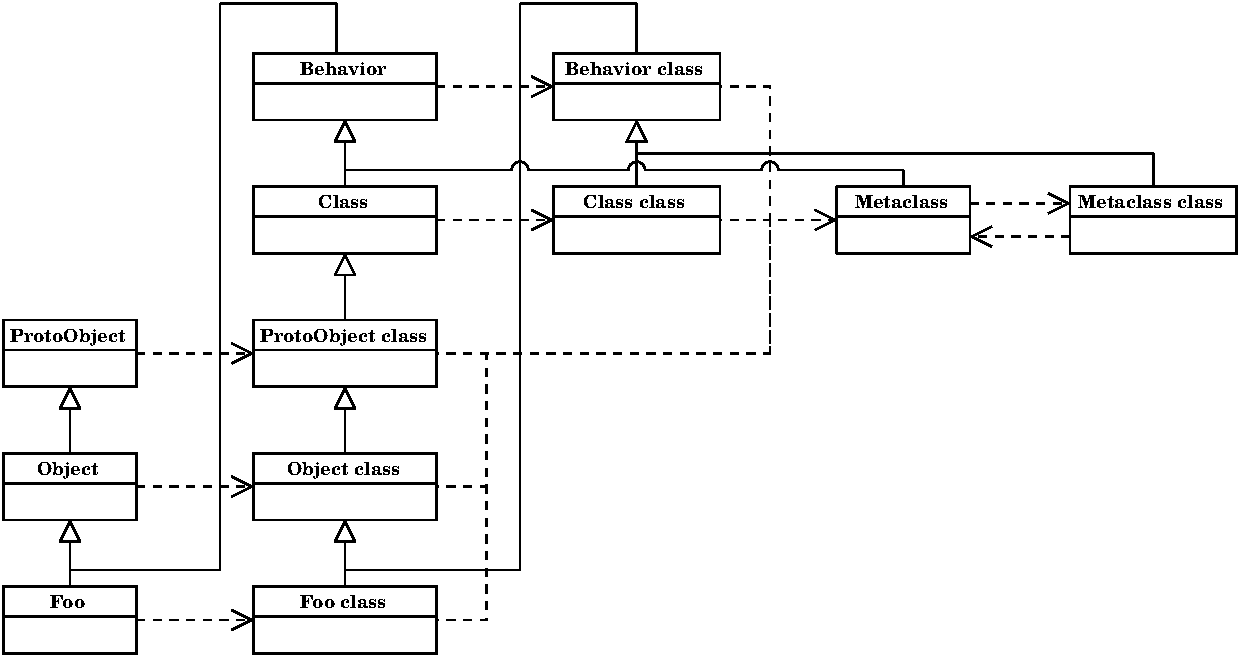
\includegraphics[width=\textwidth]{squeak_meta.pdf}
	\centering
	\caption[Squeak class model]{Squeak class model. Every class is an instance of its meta class. Meta classes are instances of \texttt{Metaclass}. Meta classes and non-meta classes form a helix~\cite{Briot:1989:PEM:74877.74921}, connecting the meta class hierarchy with the non-meta class hierarchy.}
	\label{fig:impl_squeak_meta}
\end{figure}

\msname allows class generation at runtime: class generator methods generate classes along with their respective meta classes. Therefore, we need a specification/blueprint that describes how a class generator method should construct a class. At first glance, it might seem logical to use meta classes; after all, a meta class is the class of a regular (non-meta) class and classes are instance generators. However, meta classes cannot be used as class object generators in a way required in our system for two reasons.

Firstly, meta classes do not have any information about their non-meta class counterpart: for example, they do not know anything about their instance methods or their instance variables. Instantiating a meta class would not generate a functional class object, which is why Smalltalk prohibits generating new instances of a meta class. In fact, the class \texttt{ClassBuilder} is used to create new classes and it always creates class objects along with their meta class objects.

Secondly, Smalltalk supports defining methods on the instance side and on the class side. Consequently, we do not only need to generate class objects but also meta class objects. All meta classes are an instance of \texttt{Metaclass}. But if we wanted to generate different meta classes, we would need different \texttt{Metaclass} classes, generating their corresponding meta classes. In some programming languages, the instance-of chain carries on infinitely; Ruby is an example~\cite{pavlata2012ruby}. However, in Smalltalk, every meta class is an instance of \texttt{Metaclass} and this is where the instance-of chain recurses: \texttt{Metaclass} is an instance of \texttt{Metaclass class}, which is an instance of \texttt{Metaclass}.

For this reason, we cannot use the Smalltalk-80 meta model to store information about nested classes and to generate new classes on the fly. We use our own simple meta model instead.

\paragraph{Nested Classes Meta Model}
Figure~\ref{fig:impl_meta_model} shows the meta model in our system. The meta model is built around specifications: there are specifications for classes, meta classes, and methods. A specification describes how its corresponding object is built. \texttt{ClassSpecification}s generate classes, \texttt{MetaclassSpecification}s generate meta classes, and \texttt{MethodSpecification}s generate methods. Since classes cannot exist without their respective meta classes, a class specification is always linked to its meta class specification and vice-versa. When a class specification is instantiated, the system generates both the class and the meta class. Meta class specifications cannot be instantiated on their own.

\begin{figure}[!htp]
	\centering
	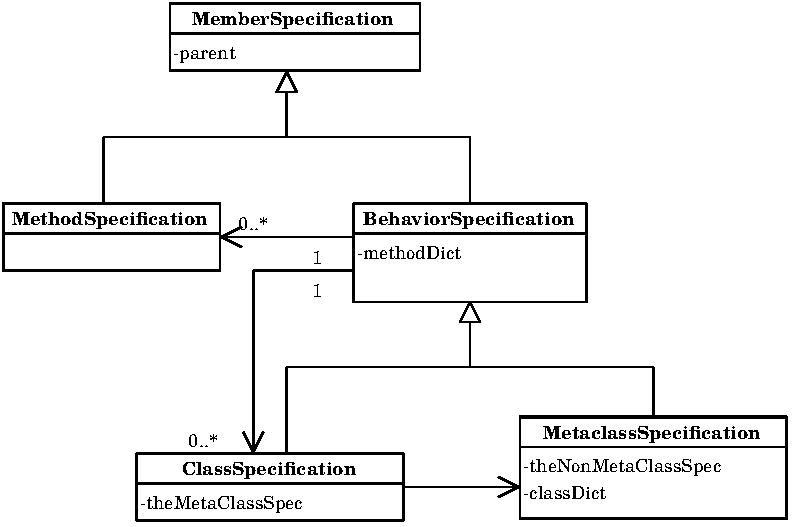
\includegraphics[scale=0.75]{metamodel.pdf}
	\caption[Meta model in \msname]{Meta model for nested classes in \msname. Class specifications are containers for method specifications. Meta class specifications can have additional nested class specifications.}
	\label{fig:impl_meta_model}
\end{figure}

\paragraph{Class Specification}
A class specification describes classes. It has a collection of \texttt{MethodSpecification}s, representing instance methods of the class. Upon instantiation, all method specifications are instantiated within the target class. For every class specification, there is a corresponding method specification containing the source code of the class generator method in the parent's\footnote{The parent of a class specification is the class specification of the enclosing class.} method dictionary. This method specification determines (when executed in the running system) to which class the methods will be added (\emph{target class}).

\paragraph{Meta Class Specification}
A meta class specification describes meta classes. It has a collection of \texttt{MethodSpecification}s, representing class methods of the class (i.e., instance methods of the meta class). Upon instantiation, all method specifications are instantiated within the target class' meta class. Consequently, there is no method specification in the parent for a meta class.

Meta classes can have nested classes of their own. For every class defined in a meta class, there is a corresponding method specification present in the method dictionary (class generator method). The class dictionary contains class specifications for nested classes.

\paragraph{Method Specification}
A method specification describes methods. It contains the source code of the method and stores information necessary for class caching and UI metadata. Whenever a method specification is instantiated, the method source code is compiled in the target class. 

Note, that different bytecode must be generated for different target classes: for example, instance variable reads and writes are compiled to parameterized\footnote{There are separate bytecodes for reading the first or second instance variable etc.} \texttt{pushRcvr:} and \texttt{popIntoRcvr:} bytecodes, where instance variables are referenced with their index\footnote{The first instance variable has index 0, the second index variable has index 1, etc.}. In addition, the \texttt{outer} and the \texttt{enclosing} keyword must be bound to different method literals, depending on the lexical scope of the method.

\paragraph{Example}
Figure~\ref{fig:impl_spec_example} shows an example of a class specification for a class \texttt{Foo}. There is a class specification for \texttt{Foo} and a meta class specification for \texttt{Foo class}. The enclosing class of \texttt{Foo} is not shown in the UML class diagram part. It is, however, shown in the meta model, because the enclosing class specification has a method specification corresponding to the class specification of \texttt{Foo}.

\begin{figure}[!htp]
	\centering
	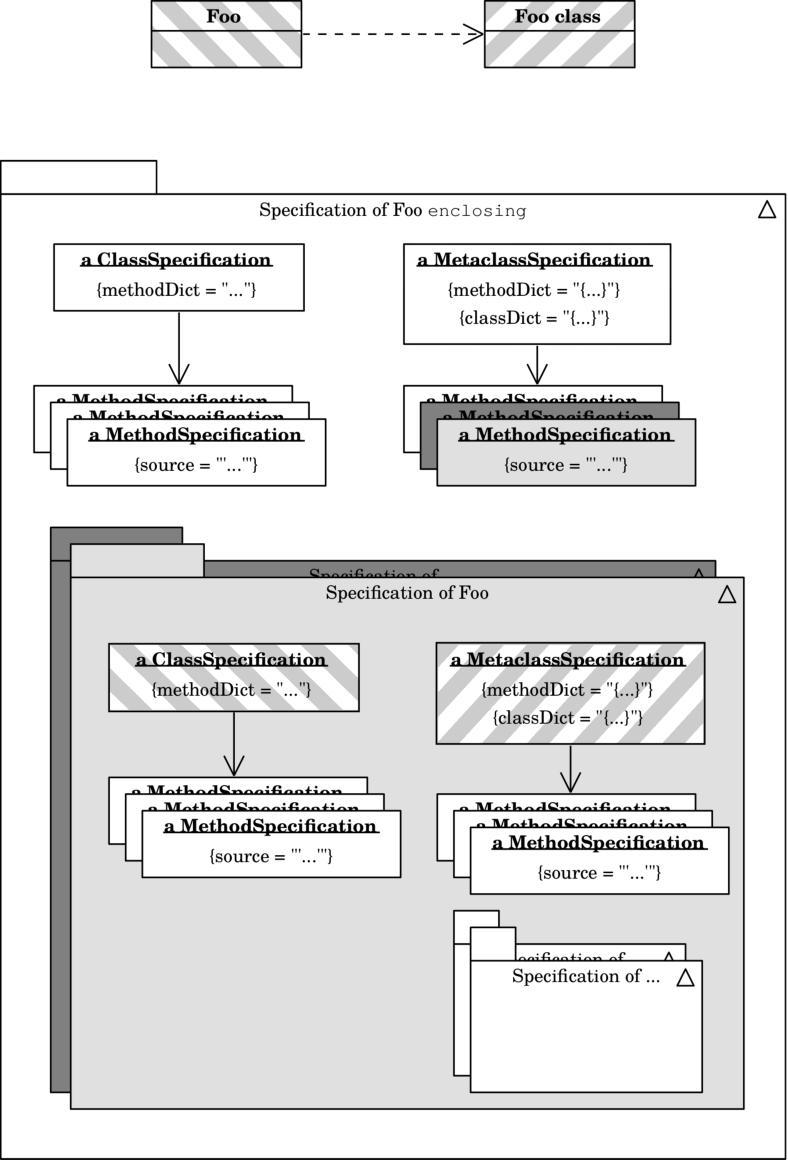
\includegraphics[width=\textwidth]{spec_example_r.pdf}
	\caption[Example: Meta model]{Example: Meta model. There is a class specification for \texttt{Foo} and a meta class specification for \texttt{Foo class} (same pattern). \texttt{Foo}'s enclosing class has a method specification (light gray color) defining the class to which the methods are added (target class), in addition to the corresponding class specification.}
	\label{fig:impl_spec_example}
\end{figure}

\section{Meta Model Instantiation}
The class specifications and meta class specifications described in Section~\ref{sec:impl_meta_model} are not class objects or meta class objects. These specifications can be instantiated, producing class objects and meta class objects. This section gives an overview of how \msname generates Smalltalk classes based on class specifications. We distinguish between \emph{class definitions} and \emph{class extensions}. In the former case, the nested class is a newly-generated subclass. In the latter case, an already existing class is extended (extension methods) or aliased. 

\subsection{Class Definitions}
In this subsection, we consider the most likely case that a brand new class is defined as a nested class, i.e., the nested class is a \emph{class definition}. Figure~\ref{fig:lazy_class_gen} illustrates how the system generates and initializes a class (class specification instantiation). 

\begin{figure}[!hbp]
	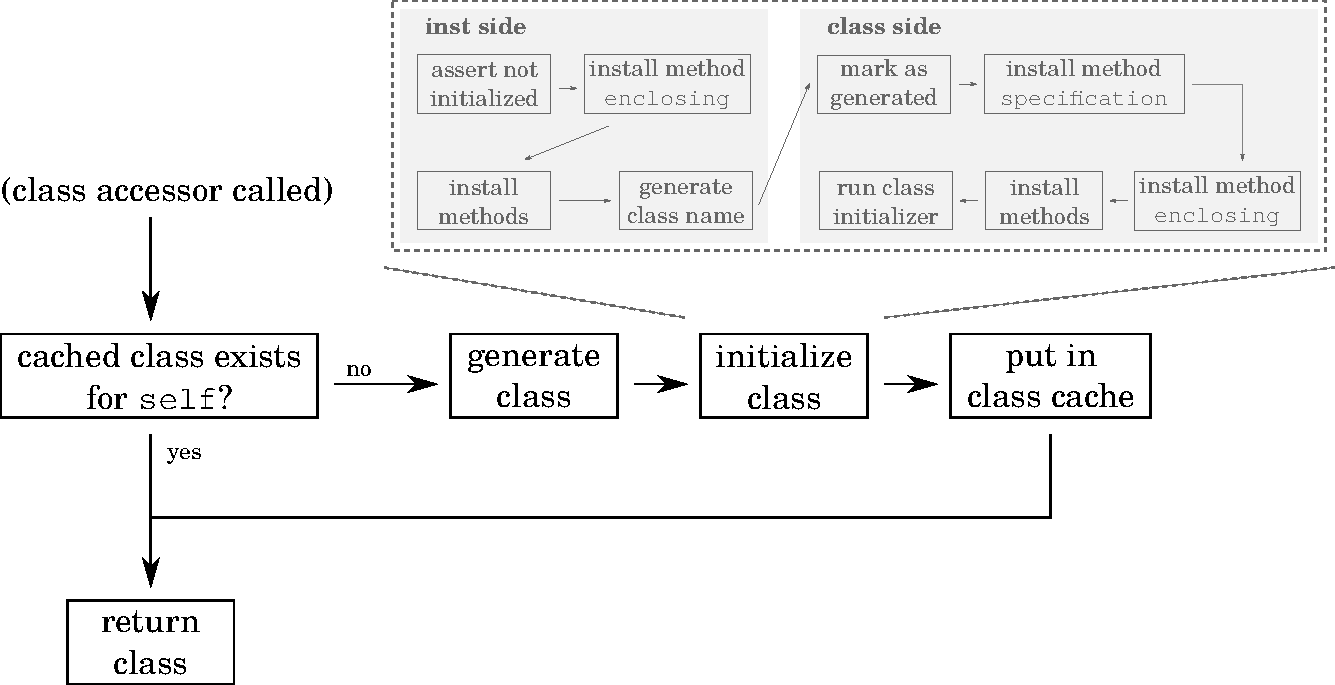
\includegraphics[width=\textwidth]{lazy_class_gen.pdf}
	\centering
	\caption[Nested class definition initialization]{Nested class definition initialization. Classes are generated lazily and initialized using a class specification and a meta class specification.}
	\label{fig:lazy_class_gen}
\end{figure}

Whenever a class accessor method is invoked, the method first checks if the class is already cached. If that is the case, it is returned. Otherwise, the class generator method is called, returning an empty uninitialized class, i.e., all instance methods are still missing and only the superclass and the instance and class variables are set up correctly\footnote{The class generator method can return any class object, but we consider only class definitions.}. The following list gives an overview of the steps necessary for initializing a class.

\begin{enumerate}
	\item Install \texttt{enclosing} instance method. This method returns the enclosing class (bound as a method literal). Note, that the enclosing class cannot be stored in an instance variable of the nested class, because \texttt{enclosing} should be early bound and \texttt{super enclosing} should return a class different from \texttt{self enclosing}, in case the superclass of the nested class has a different enclosing class.
	\item Install/compile all instance methods listed in the class specification.
	\item Generate the class name. The class name is a concatenation of the enclosing class' name and the selector of this class' accessor method. It is stored as an instance variable on \texttt{Class}. Note, that every class object is an instance of its meta class, which is a subclass of \texttt{Class} (Figure~\ref{fig:impl_squeak_meta}).
	\item Add a marker method to the meta class to mark it as generated. This makes it easy to check if a class is an ordinary (legacy) Smalltalk class or was generated within \msname.
	\item Install \texttt{specification} class method. This method returns the class specification (bound as a method literal), which is useful for meta programming purposes. Note, that the specification cannot be stored in an instance variable of the class, because \texttt{specification} should be early bound and \texttt{self specification} should return a specification different from \texttt{super specification}.
	\item Install \texttt{enclosing} class method. This method is identical to the instance method.
	\item Install/compile all class methods listed in the meta class specification.
	\item Send \texttt{initialize} to the class object.
\end{enumerate}

Note, that class initialization is lazy. A class is only generated and initialized if the corresponding accessor method was called. All references to classes in the source code call the corresponding accessor method, making sure that the class is available when it is needed. 

In class definitions, class generator methods always return new subclasses of other classes\footnote{See Section~\ref{sec:impl_anon_subclass} for syntax details.}; the superclass is referenced by calling its accessor method. Compared to the default package-loading process in Squeak, this makes class creation easier. In Squeak, the system has to analyze which classes are subclasses of each other, in order to create classes in the correct order (superclass has to exist before subclass is created). In our system, classes are created when their accessor methods are called, and if these classes depend on other superclasses, these superclasses are created when the class generator methods call their accessor methods (if they do not already exist).

\paragraph{Class Accessor Methods and Class Generator Methods}
For a nested class, two methods are installed on the meta class object: a class generator method, returning the class to which methods should be added (usually a newly-created subclass), and a class accessor method, checking whether the class was already created and is in the cache or calling the class generator method, otherwise.

The selector for the class accessor method is the name of the class. The selector for the class generator method is the same selector, but with a dollar sign prefix. This ensures that the method can only be called by using meta programming from our system, and avoids accidential name clashes with other methods. For example, if a class is named \texttt{Foo}, the class accessor method has the selector \texttt{Foo} and the class generator method has the selector \texttt{\$Foo}.

\subsection{Class Extension}
\label{sec:impl_class_ext_subsec}
Whenever the class generator method for a nested class returns an already existing class that is already initialized, we call the nested class a \emph{class extension}. Class extensions are useful to extend inherited nested classes without subclassing (see Section~\ref{sec:concept_inh_nested_cl}) and to declare extensions methods (see Section~\ref{sec:usecases_ext_meth}). 

The process of class initialization for class extensions (Figure~\ref{fig:lazy_class_gen_ext}) is easier than the process for class definitions: there are no \texttt{enclosing} methods installed and no new class name is generated. The already existing \texttt{specification} methods are modified, such that they return an array of specifications. If a class is extended multiple times, this array contains all corresponding class specifications. The first specification in the array is always the specification where the class was defined.

\begin{figure}[!htp]
	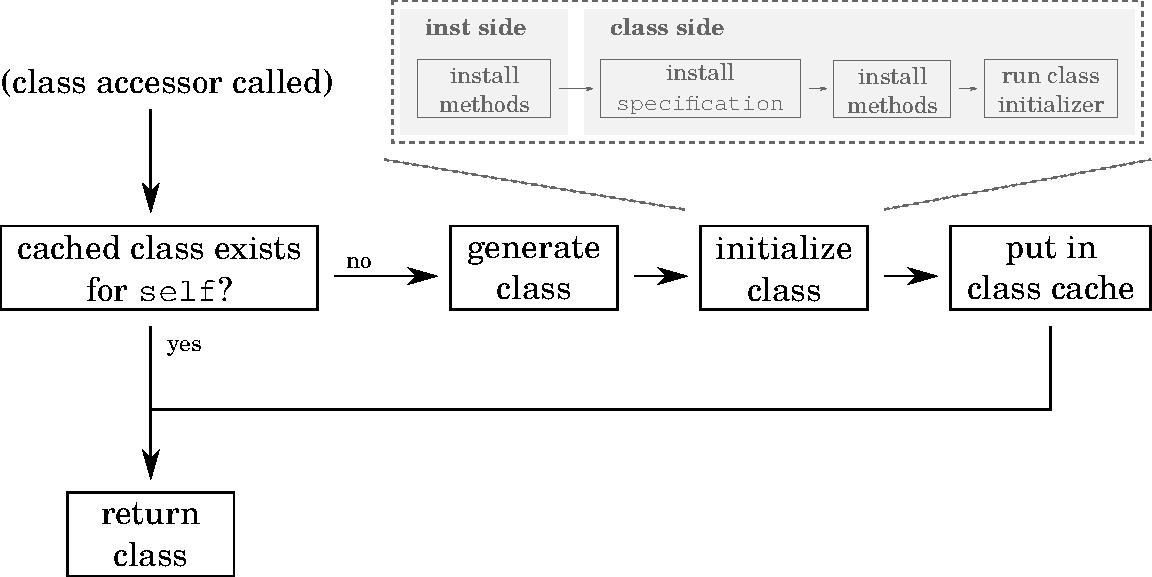
\includegraphics[width=0.8314\textwidth]{lazy_class_gen_ext.pdf}
	\centering
	\caption[Nested class extension initialization]{Nested class extension initialization. An already existing and initialized class is initialized.}
	\label{fig:lazy_class_gen_ext}
\end{figure}

\section{Anonymous Classes and Subclass Generation}
\label{sec:impl_anon_subclass}
In Smalltalk, new classes are created by subclassing an already existing class. Squeak has a special class, the \texttt{ClassBuilder}, containing all the functionality for creating the class object, the meta class object, giving the class a name, possibly migrating the old class and its instances (if an existing class was changed), and registering it in the \texttt{globals} dictionary.

\msname reuses the class builder and adds functionality for creating anonymous subclasses. Anonymous subclasses~\cite{Ducasse99evaluatingmessage} do not have a name and certain checks are omitted (e.g., if the class name starts with a capital letter). Also, anonymous subclasses are not added to the \texttt{globals} dictionary.

\paragraph{Subclass Notation}
Figure~\ref{fig:impl_subclass_squeak} shows how subclasses are created in Squeak. The first statement is a message send to \texttt{Object} which not only creates the subclass but also adds it to the \texttt{globals} dictionary. The second statement is also executable code that adds an instance variable to the meta class object. The difference between class variables and class instance variables is that class variables are shared among all subclasses, whereas class instance variables have different values for every class object~\cite{classvar1,classvar2}. For example, if \texttt{A} has a class variable \texttt{Bar} and \texttt{B} is a subclass of \texttt{A}, then both \texttt{A} and \texttt{B} share one variable \texttt{Bar}.

\begin{figure}[!htp]
\begin{subfigure}[b]{\textwidth}
\begin{lstlisting}
Object subclass: #NewClass
    instanceVariableNames: <@\textcolor{RoyalPurple}{'foo bar'}@>
    classVariableNames: <@\textcolor{RoyalPurple}{'Bar'}@>
    poolDictionaries: <@\textcolor{RoyalPurple}{''}@>
    category: <@\textcolor{RoyalPurple}{'Demo-Experiments'}@>.

NewClass class
	instanceVariableNames: <@\textcolor{RoyalPurple}{'Foo'}@>.
\end{lstlisting}
\caption{Subclass notation in Squeak}
\label{fig:impl_subclass_squeak}
\end{subfigure}

\vspace{15pt}

\begin{subfigure}[b]{\textwidth}
\begin{lstlisting}
<@\textbf{NewClass}@>
    <@\textcolor{OliveGreen}{\textbf{< class >}}@>
    ^ Object 
        subclassWithInstVars: <@\textcolor{RoyalPurple}{'foo bar'}@>
        classVars: <@\textcolor{RoyalPurple}{'Bar'}@>
        classInstVars: <@\textcolor{RoyalPurple}{'Foo'}@>
\end{lstlisting}
\caption{Subclass notation with nested classes}
\label{fig:impl_subclass_nested}
\end{subfigure}
\caption[Notation for creating subclasses]{Full notation for creating subclasses. \msname provides abbreviations (convenience methods) in case no additional instance variables or class variables should be defined (e.g., \texttt{subclass}).}
\end{figure}

Figure~\ref{fig:impl_subclass_nested} shows how subclasses are created in \msname. \texttt{NewClass} is a class generator method and also the name of the new class. Therefore, it is no longer necessary to pass a symbol with the name of the new class to the \texttt{subclass:} method. Note, that the \texttt{<class>} pragma is necessary to distinguish between class generator methods and regular methods, which might accidentially return a class. Only in the former case, a class specification object is created.

\section{Implementation of Keywords}
\label{sec:impl_keywords}
In this section, we explain how the keywords \texttt{enclosing}, \texttt{outer}, and \texttt{scope} are implemented. All message sends to \texttt{enclosing} are forwarded to the enclosing class. All message sends to \texttt{outer} are forwarded all enclosing classes consecutively, whenever a class does not understand the message. All message sends to \texttt{scope} are first treated as \texttt{self} sends, then as sends to \texttt{outer}.

\paragraph{Implementation of \texttt{enclosing}}
During compilation, all references to \texttt{enclosing} are bound to the enclosing class, which is known during class initialization. Technically, every class has its own Squeak environment which binds \texttt{enclosing} to the enclosing class. Therefore, it is also possible to evaluate \texttt{enclosing} in the debugger, for example.

\paragraph{Implementation of \texttt{outer}}
During compilation, all references to \texttt{outer} are bound to an instance of \texttt{LexicalScope}. This class is a subclass of \texttt{ProtoObject}, holds references to all enclosing classes in the lexical scope, and contains a \texttt{doesNotUnderstand:} handler, that forwards messages to the enclosing classes. If the enclosing class does not understand the message, the message is forwarded to the next enclosing class\footnote{The lexical scope of a method can only be determined by analyzing the structure of the meta model. For more details, see Section~\ref{sec:app_lexical_scope}.}. If at some point, a top-level class without an enclosing class is reached, the handler looks for an entry in the \texttt{globals} dictionary with the message's selector.

\afterpage{%

\begin{figure}[!htp]
\vspace{50pt}
\begin{subfigure}[b]{\textwidth}
	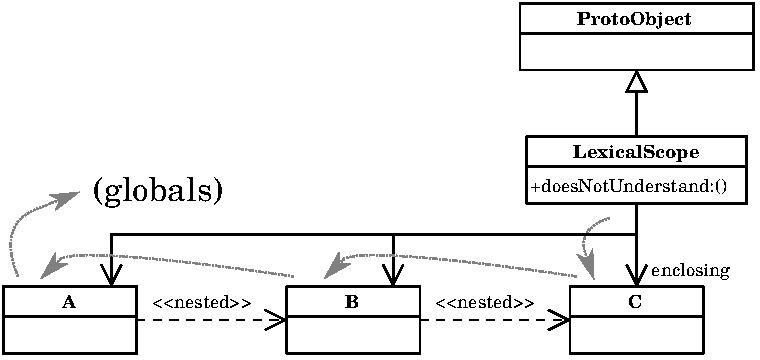
\includegraphics[scale=1]{lexical_outer.pdf}
	\centering
	\caption{\texttt{LexicalScope} for \texttt{outer} keyword}
	\label{impl:lex_outer}
\end{subfigure}

\vspace{35pt}

\begin{subfigure}[b]{\textwidth}
	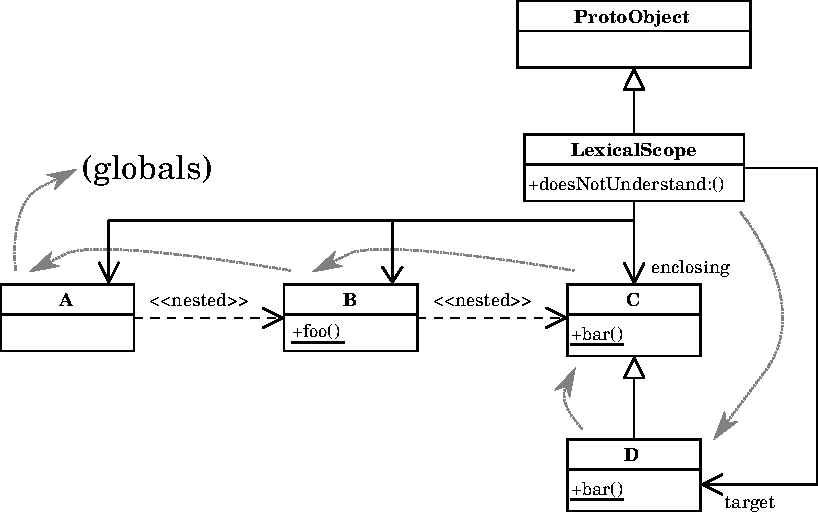
\includegraphics[scale=1]{lexical_scope.pdf}
	\centering
	\caption{\texttt{LexicalScope} for \texttt{scope} keyword}
	\label{impl:lex_scope}
\end{subfigure}
\vspace{10pt}
\caption[Example: Method lookup with \texttt{LexicalScope}]{Example: Method lookup using \texttt{LexicalScope}. Message sends to \texttt{scope} have an additional \texttt{target} object involved in the lookup, which is the receiver class in the context where \texttt{scope} appears in the source code. All association arrows actually reference the class object.}
\end{figure}
\clearpage
}

As an example, let us assume that we have classes nested as shown in Figure~\ref{fig:concept_nested_notation} and that all following message sends to \texttt{outer} happen in \texttt{A class>>B class>>C class>>m4}. See Figure~\ref{impl:lex_outer} for a visualization of the lookup.
\begin{itemize}
	\item \texttt{outer foo}: lookup in \texttt{enclosing at: 1} (class \texttt{A B}) succeeds.
	\item \texttt{outer B}: lookup in \texttt{enclosing at: 1} fails, but lookup in \texttt{enclosing at: 2} (class \texttt{A}) succeeds.
	\item \texttt{outer A}: lookup in \texttt{enclosing at: 1} and \texttt{enclosing at: 2} fails, but \texttt{A} is present in the \texttt{globals} dictionary.
	\item \texttt{outer Object}: same as before. All classes outside of our system are also present in the \texttt{globals} dictionary.
	\item \texttt{outer D}: lookup fails and raises a \texttt{MessageNotUnderstood} error.
\end{itemize}

\paragraph{Implementation of \texttt{scope}}
References to \texttt{scope} cannot be replaced by a constant literal during compile time. This is because the lookup involves a lookup in \texttt{self}\footnote{If \texttt{scope} is used in an instance method, the lookup starts at \texttt{self class}.}. Looking up methods in the class of the method under compilation is not sufficient, because that method might be overridden in a subclass\footnote{\texttt{self} sends are late bound.}. Therefore, we have to construct a \texttt{LexicalScope} object at runtime (instead of compile time) and pass it two objects: the array of all enclosing classes (contained in \texttt{outer}) and \texttt{self}.

Figure~\ref{impl:lex_scope} shows how the \texttt{scope} lookup works in a slightly modified example. Just as in the previous example, we assume that all message sends happen in \texttt{A class>>B class>>C class>>m4}. However, \texttt{m4} is invoked on class \texttt{D}, which is a subclass of class \texttt{A B C}. Therefore, \texttt{self} is bound to \texttt{D}.

\begin{itemize}
	\item \texttt{scope bar}: lookup in \texttt{self} succeeds: method \texttt{D class>>bar}.
	\item \texttt{scope foo}: lookup in \texttt{self} fails, but lookup in \texttt{enclosing at: 1} (class \texttt{A B}) succeeds.
	\item The lookup for all other examples listed for \texttt{outer} (previous paragraph) yields the same result in this example.
\end{itemize}

Note, that the reference to \texttt{self} (\texttt{target}) cannot be established at compile time, because it is unclear what the polymorphic receiver class is. Therefore, references to the keyword \texttt{scope} have to be replaced by a message send: \texttt{LexicalScope for: self in: outer}. This has the side effect that the decompiled source code (and the code shown in the debugger) looks slightly different from the code written by the programmer.

\section{Class Caching}
\label{sec:impl_class_cache}
Whenever a nested class is accessed, the class accessor method checks if the class was already generated. If that is the case, the cached version of the class is returned. For this reason, every class specification with a unary selector (unparameterized class) has an instance variable \texttt{classCache}, which contains cached class objects. 

\paragraph{Caching Unparameterized Classes}
\texttt{classCache} is a dictionary mapping enclosing class objects to nested class objects. Every unparameterized class object can only have one instantiation. However, consider, for example, the situation in Figure~\ref{fig:impl:subclass_inherited_class}. In this case, \texttt{A2} caches two instances of \texttt{B}: one for \texttt{A1 class>>B} (created and cached during the \texttt{super B} call) and one for \texttt{A2 class>>B}. The former one contains only the methods defined in \texttt{A1 class>>B}. The latter one is a subclass of the former one and contains all methods defined in \texttt{A2 class>>B}. In this example, the corresponding class specification for \texttt{A2 class>>B} has a class cache mapping \texttt{A1} to the former one and mapping \texttt{A2} to the latter one.

\paragraph{Parameterized Classes}
The system does not cache parameterized classes, as this could result in an excessive number of classes being kept around. One can argue, that a nested weak identity key dictionary data structure could solve this problem: \texttt{classCache} is a \texttt{WeakIdentityKeyDictionary}, whose keys are the first argument. The values are again \texttt{WeakIdentityKeyDictionary}s, mapping the second argument to \texttt{WeakIdentityKeyDictionary}s. Eventually, the last argument is mapped to class objects instead of dictionaries (Figure~\ref{fig:impl_class_cache}).

\begin{figure}[!htp]
	\begin{minipage}{\textwidth}
	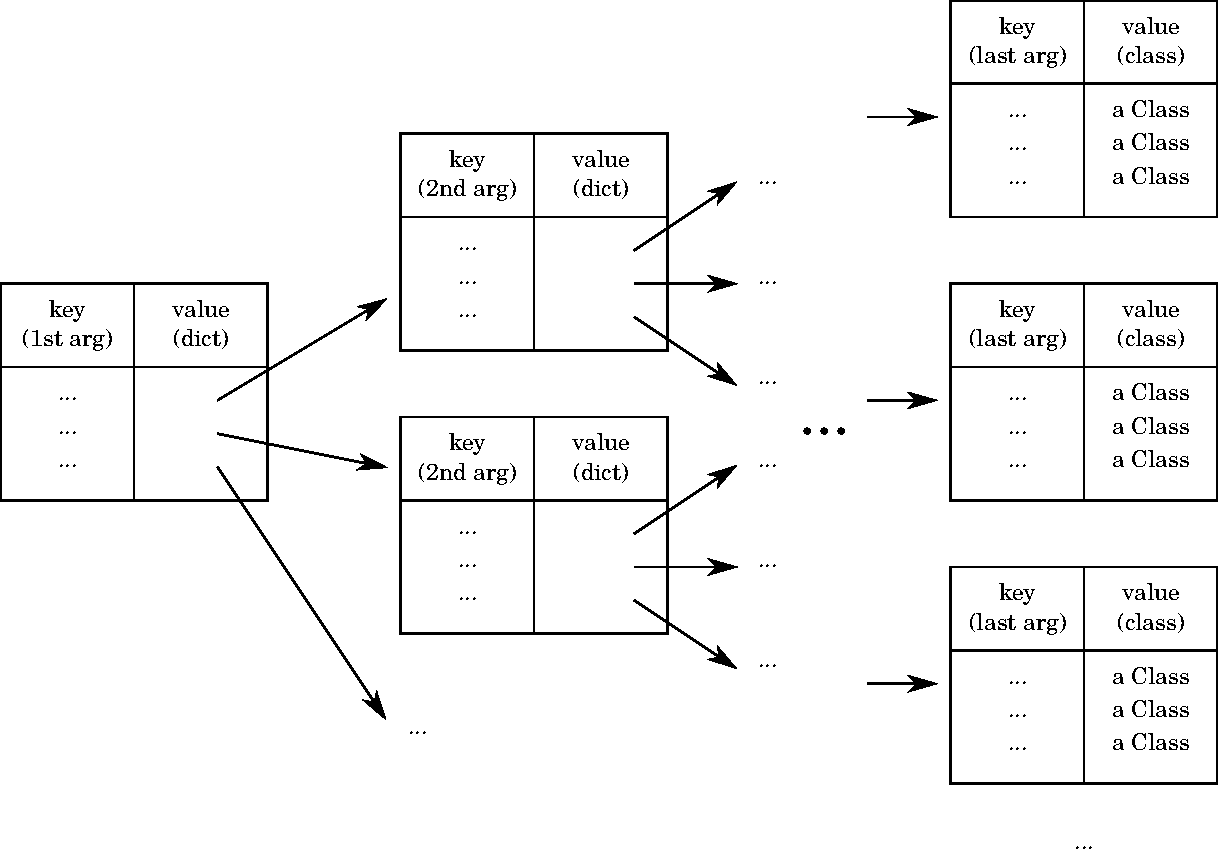
\includegraphics[width=\textwidth]{class_cache.pdf}
	\centering
	\caption[Class cache for parameterized classes]{Class cache for parameterized classes. The cache is a nested dictionary data structure, with an additional level of nesting per parameter.}
	\label{fig:impl_class_cache}
	\end{minipage}
	\begin{minipage}{\textwidth}
	\vspace{30pt}
	\begin{lstlisting}
<@\textbf{MyLibrary class>>BaseClass}@>
    <@\textcolor{OliveGreen}{\textbf{< class >}}@>
    " This is the class that serves as 
      an input for the mixin in this example. "
	

<@\textbf{MyLibrary class>>CollectionMixin:}@> base
    <@\textcolor{OliveGreen}{\textbf{< class >}}@>
    " This class is uncached because it is parameterized "

    ^ base subclass


<@\textbf{MyLibrary class>>MyCollection}@>
    <@\textcolor{OliveGreen}{\textbf{< class >}}@>
    " This is the cached mixin application. "

    ^ self CollectionMixin: self BaseClass
\end{lstlisting}
\caption[Cached mixin application]{Example: Cached mixin application. The mixin application is uncached, because the mixin is a parameterized class. However, the aliased mixin application \texttt{MyCollection} is cached, because it is an unparameterized class.}
\label{fig:impl_cached_mixin_application}
\end{minipage}
\end{figure}

In this case, class objects are garbage collected once there is no reference to at least one of the arguments in the system anymore. However, it depends on how exactly parameterized classes are used. If parameterized classes are used heavily, for example with \texttt{SmallInteger}s as parameters (or other globally reachable objects), no class would ever be garbage collected, because \texttt{SmallInteger}s are represented as tagged objects in Squeak~\cite{Bolz:2008:BFO:1482373.1482382, papetechreport}. If parameterized classes are used as mixins, this is arguably less of a problem, because the number of base classes to which a mixin is applied is usually not excessively large. However, note, that mixin applications can easily be cached by aliasing them as an unparameterized class (Figure~\ref{fig:impl_cached_mixin_application}). We argue that mixins will most of the time be used in such a way, because writing the mixin application explicitly is more verbose and hinders readability; in addition, the programmer might want to add additional methods to the mixin application, in which case the mixin application must be subclassed or aliased as described, anyway.

\section{Class Updates}
Squeak is a live programming environment with immediate feedback. When the programmers changes a class, these changes should immediately affect all instances of the class in the system, i.e., existing instances must be migrated to the new class~\cite{casaccio2011bootstrapping}. In that sense, Squeak and many other Smalltalk implementations~\cite{Penney:1987:CMG:38765.38817} are different from other programming languages with an ``edit/compile/run cycle''~\cite{conf/sofsem/NierstraszG10}: the programmer has the feeling that there is no difference between compile time and runtime.

For this reason, \msname has to ensure that changes to the source code are immediately applied to all living objects in the image. It is important to understand, that changes to parameterized class specifications can affect multiple classes (model instantiations) at runtime. Therefore, every class specification stores a weak collection of all its instantiations (\texttt{instantiations}). This collection is in fact a \texttt{WeakIdentityKeyDictionary} and also used to cache arguments for parameterized classes (see Section~\ref{sec:impl_migration}). When a class specification is changed, all of its instantiations can be looked up easily and adapted one by one. Note, that this dictionary is different from the class cache, as it holds on to instantiations weakly.

\subsection{Changing Instance/Class Methods}
Whenever an instance method is added, removed, or changed, the system retrieves the collection of all instantiations, and performs the corresponding change on the class object. This does not require creating a new class object, but merely changing the method dictionary using Squeak's meta object protocol~\cite{Goldberg:1983:SLI:273, Kiczales:1991:AMP:574212}.

Changing class methods is equivalent to changing instance methods, with the only difference being that the meta class object is changed instead of the class object.

\subsection{Changing Instance/Class Variables}
This kind of class change is more difficult to handle than method changes. Whenever an instance/class instance variable is added or removed, some methods might have to be recompiled, because instance variables are referenced with indices in the bytecode (see also Section~\ref{sec:impl_meta_model}). 

\paragraph{Instance Variables Indexing}
\begin{figure}[!htp]
	\centering
	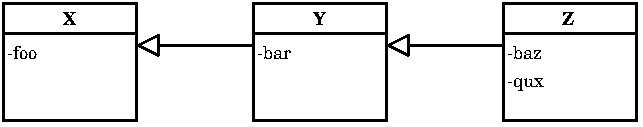
\includegraphics[scale=1]{inst_vars.pdf}
	\caption[Example: Instance variables indexing]{Example: Instance variables indexing. Every instance variable has a zero-based index. The index of inherited instance variables is preserved.}
	\label{fig:impl_inst_vars}
\end{figure}

In Figure~\ref{fig:impl_inst_vars}, class \texttt{X} has instance variable \texttt{foo}, class \texttt{Y} has instance variables \texttt{foo} and \texttt{bar}, and class \texttt{Z} has instance variables \texttt{foo}, \texttt{bar}, \texttt{baz}, and \texttt{qux}. Instance variables are indexed according to the superclass hierarchy. Therefore, \texttt{foo} has index 0, \texttt{bar} has index 1, \texttt{baz} has index 2, and \texttt{qux} has index 3. These indices are used in the bytecode instead of string literals or symbols. Therefore, when instance variables are changed in \texttt{X}, all classes (methods referencing these instance variables) \texttt{X}, \texttt{Y}, and \texttt{Z} have to be recompiled. If instance variables in \texttt{Z} are changed, only \texttt{Z} has to be recompiled.

\paragraph{Definition of Instance Variables}
What is more interesting is how instance variables are defined in \msname: they are part of the class generator method (Figure~\ref{fig:impl_subclass_nested}). Therefore, the system has to execute that method a second time whenever it is changed. The method returns a new class object which must be initialized again, i.e., all methods are recompiled. Squeak has the same behavior: whenever an instance variable is changed, methods in the current class and all subclasses are recompiled. Section~\ref{sec:impl_migration} gives an overview of the steps necessary for class migration.

\subsection{Changing Target Class}
The target class is the class that is returned by the class generator method. It is usually a new subclass. The superclass of a nested class can be changed by changing the receiver of the \texttt{subclass} message in the class generator method. Whenever the target class is changed, the class generator method must be executed a second time and the old class must be migrated to the new one. From a class migration point of view, it does not matter whether an instance variable or the target class was changed. The same class migration process follows.

\subsection{Class Migration}
\label{sec:impl_migration}
Whenever an instance variable or the target class in a class generator method is changed, the changed class generator method must be executed a second time and the old class object must be migrated to the new class object. In this subsection, we describe some of the pitfalls in this process.

\paragraph{Class Argument Cache}
\label{sec:impl_cls_arg_cache_subsec}
\begin{figure}[!htp]
	\centering
	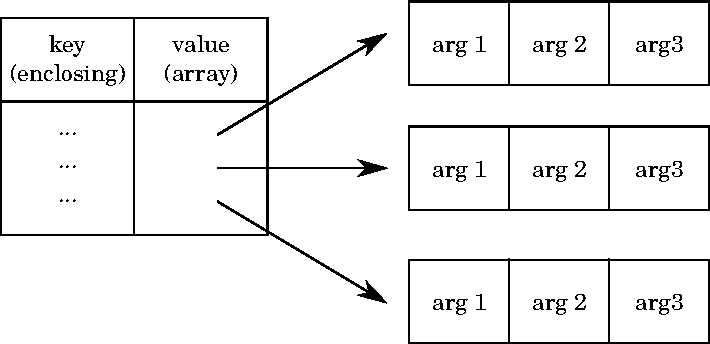
\includegraphics[scale=0.7]{arg_cache.pdf}
	\caption[Example: Argument cache]{Example: Argument cache. The cache is a dictionary mapping parameterized instantiations to an array of arguments that was used to generate the respective class.}
	\label{fig:impl_arg_cache}
\end{figure}

Class generator methods for unparameterized classes can just be invoked without any parameters. However, in order to update parameterized classes, the system has to cache the arguments provided to the class generator method when the class was generated. Therefore, every class specification maintains an argument cache (\texttt{instantiations}), mapping instantiations (classes) to an array of arguments and the class that owns the nested class\footnote{The owner class is not necessarily the enclosing class. The enclosing class is early bound, whereas the owner is the class to which the class accessor selector was sent.}. This argument cache is a \texttt{WeakIdentityKeyDictionary} and different from the dictionary data structure shown in Figure~\ref{fig:impl_class_cache}. That class cache would map arguments to instantiations. Whenever there is no reference to an instantiation in the image anymore, the array of arguments can be garbage collected, because nobody can access the class anymore; therefore, this class does not have to be updated.

\paragraph{Class Migration}
Invoking the class generator method a second time usually generates a new class\footnote{There are exceptions: for example, executing the method for an alias a second time does not generate a new class.}. Therefore, all references to the old class have to be replaced with references to the new class using the \texttt{becomeForward:} method. Also, all instances of the old class have to be migrated to the new class. This is no different from what Squeak does when an instance variable is added or removed, and not described in any more detail in this work. We encourage the reader to consult the \emph{Smalltalk Blue Book}~\cite{Goldberg:1983:SLI:273} for more information.

At this point, we have to distinguish between class definitions and class extensions. We always migrate classes for a class definition. However, not all class extensions are migrated. Consider, for example, the case that the programmer created an alias for \texttt{String} and changed that alias to point to \texttt{SmallInteger}. In this case, we should not migrate all instances of \texttt{String} to \texttt{SmallInteger}. The rationale behind this example is that aliases and class extensions can be applied at multiple points throughout the program. Classes should never be migrated when such a class is changed, because other (unchanged) points in the program will be affected. 

\begin{figure}[!htp]
\centering
\begin{subfigure}[b]{0.45\textwidth}
\begin{lstlisting}
<@\textbf{MyClass}@>
    <@\textcolor{OliveGreen}{\textbf{< class >}}@>
    ^ Object
\end{lstlisting}
\caption{Class extension}
\label{fig:impl_cls_migr_ext}
\end{subfigure}
\qquad
\begin{subfigure}[b]{0.45\textwidth}
\begin{lstlisting}
<@\textbf{MyClass}@>
    <@\textcolor{OliveGreen}{\textbf{< class >}}@>
    ^ Object subclass
\end{lstlisting}
\caption{Class definition}
\label{fig:impl_cls_migr_def}
\end{subfigure}

\vspace{10pt}

\begin{subfigure}[b]{0.45\textwidth}
\begin{lstlisting}
<@\textbf{MyClass}@>
    <@\textcolor{OliveGreen}{\textbf{< class >}}@>
    ^ super MyClass
\end{lstlisting}
\caption{Class extension \\ (extending inherited nested class)}
\label{fig:impl_cls_migr_ext_nested}
\end{subfigure}
\qquad
\begin{subfigure}[b]{0.45\textwidth}
\begin{lstlisting}
<@\textbf{MyClass}@>
    <@\textcolor{OliveGreen}{\textbf{< class >}}@>
    ^ super MyClass subclass
\end{lstlisting}
\caption{Class definition \\ (subclassing inherited nested class)}
\label{fig:impl_cls_migr_subclass_nested}
\end{subfigure}
\caption[Example: Class migration]{Example: Class migration. In (b) and (d), a class is defined. Therefore, these classes will be migrated. In (a), a class is aliased. This class will not be migrated. In (c), a class defined in the same object (\texttt{self}) where it is extended, so this class will be migrated. We assume that the superclass in (c) actually defines the class and does not extend a class.}
\label{fig:impl_cls_migration_full}
\end{figure}

There is one exception to this rule. Whenever an inherited nested class is extended in a subclass, the class should be migrated, because every subclass has its own nested class that is different from the superclass' nested class, even though the nested class is defined in the superclass and extended in the subclass. Therefore, class extensions are migrated, only if the original class definition took place in the same object as the class extension in question.

Figure~\ref{fig:impl_cls_migration_full} shows multiple examples. Figure~\ref{fig:impl_cls_migr_ext_nested} is the interesting case. An inherited nested class is extended. We assume, that the enclosing superclass defined \texttt{MyClass}. In that case, \texttt{MyClass} is defined in the same class as it is extended: it is defined in \texttt{super MyClass} and extended in \texttt{self MyClass} (same receiver in both cases).

\paragraph{Clearing Class Extension Caches}
Whenever a class is migrated, all class extensions have to be reapplied. During class migration, \texttt{becomeForward:} is used to replace all references to the old class with references to the new class, including class caches. After class migration, all class caches for class extensions for the new class are cleared. When the migrated class is later accessed through an alias or a class extension, all extension methods are reapplied.

\paragraph{Changing Class Extensions}
Whenever the class generator method for a class extension is changed, \msname first undoes all changes to affected classes, i.e., it removes all methods that were added or replaced. It does at the moment not restore replaced methods. Colliding extension methods are a known problem in Smalltalk. Other techniques have been proposed, but are out of scope for this thesis (see Section~\ref{sec:future_ext_meth}). After changes to to affected classes have been undone, \msname clears the class cache. Therefore, all class extensions are reapplied when the class is accessed again through the accessor method for the class extension. In case the class extension is an extension of an inherited nested class, the migration process takes place as previously described.

\paragraph{Overview}
Figure~\ref{fig:impl_update_cycle} gives a high-level overview of the entire class migration process.

\begin{figure}[!htp]
	\centering
	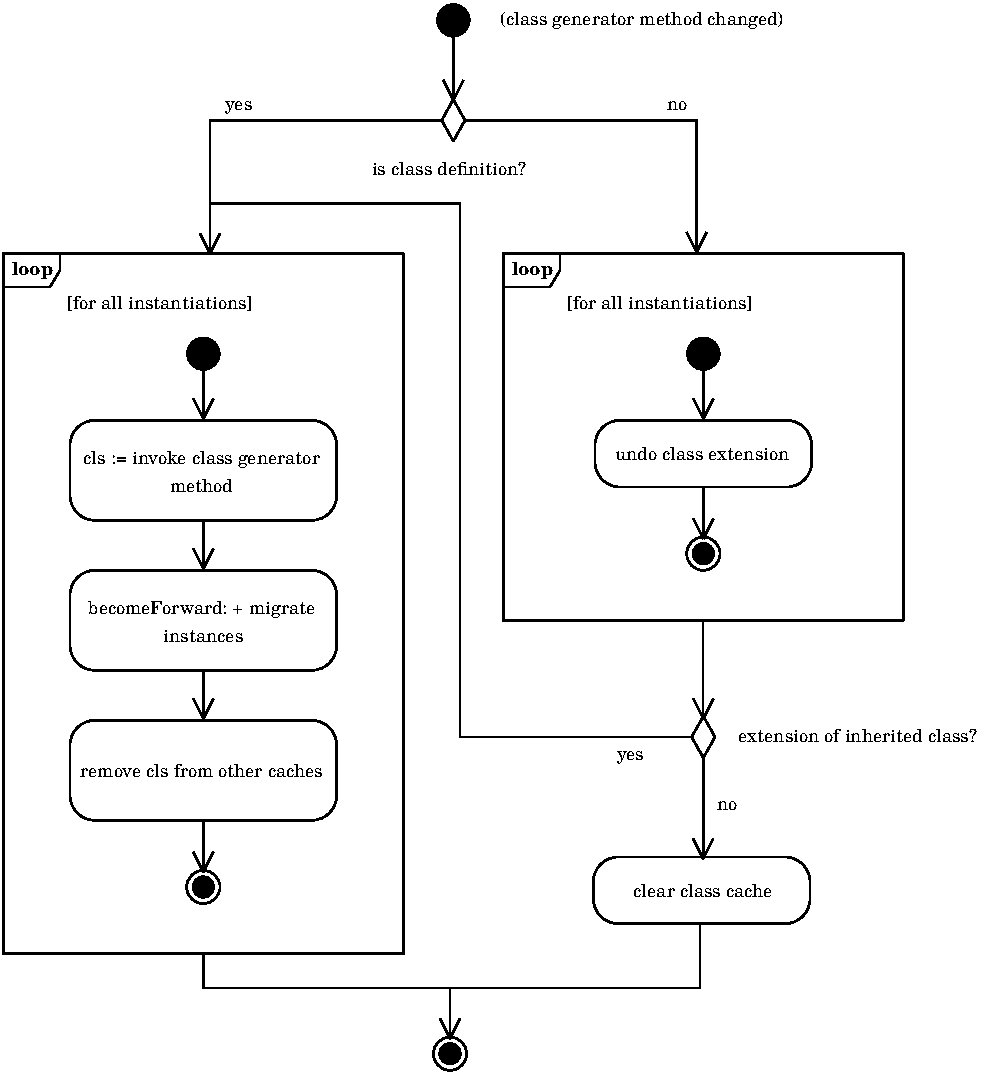
\includegraphics[width=\textwidth]{update_cycle.pdf}
	\caption[Class migration process]{High-level overview of the class migration process. Classes and instances are only migrated if the nested class is a class definition or a class extension of an inherited nested class.}
	\label{fig:impl_update_cycle}
\end{figure}

\section{Integration in Squeak}
In this section, we describe how \msname is integrated in Squeak.

\subsection{Module Repository}
At the moment, there is a separate \emph{module repository} for \msname. This is a singleton class with a collection all top-level class specifications and a collection of instantiated top-level class specifications. This is useful for development purposes, because basic Squeak classes can be migrated to our system without the risk of damaging the base system. References to classes are first looked up in the module repository, then in the Smalltalk \texttt{globals} dictionary.

Eventually, all classes written in \msname should be listed in the Smalltalk \texttt{globals} dictionary, replacing system classes with their counterparts written in \msname, which would also make the module repository obsolete.

\subsection{IDE Support}
\msname comes with a proof-of-concept implementation of a class browser. The existing system browser cannot be used, because it cannot handle class nesting. Our class browser is written in Vivide~\cite{Taeumel:2012:VPE:2384592.2384604}, a framework for dataflow-driven tool development, and shown in Figure~\ref{fig:impl_class_browser}. It supports creating and deleting methods and nested classes, but basic refactoring functionality and functionality such as browsing senders and receivers is still missing.

\begin{figure}[!htp]
	\centering
	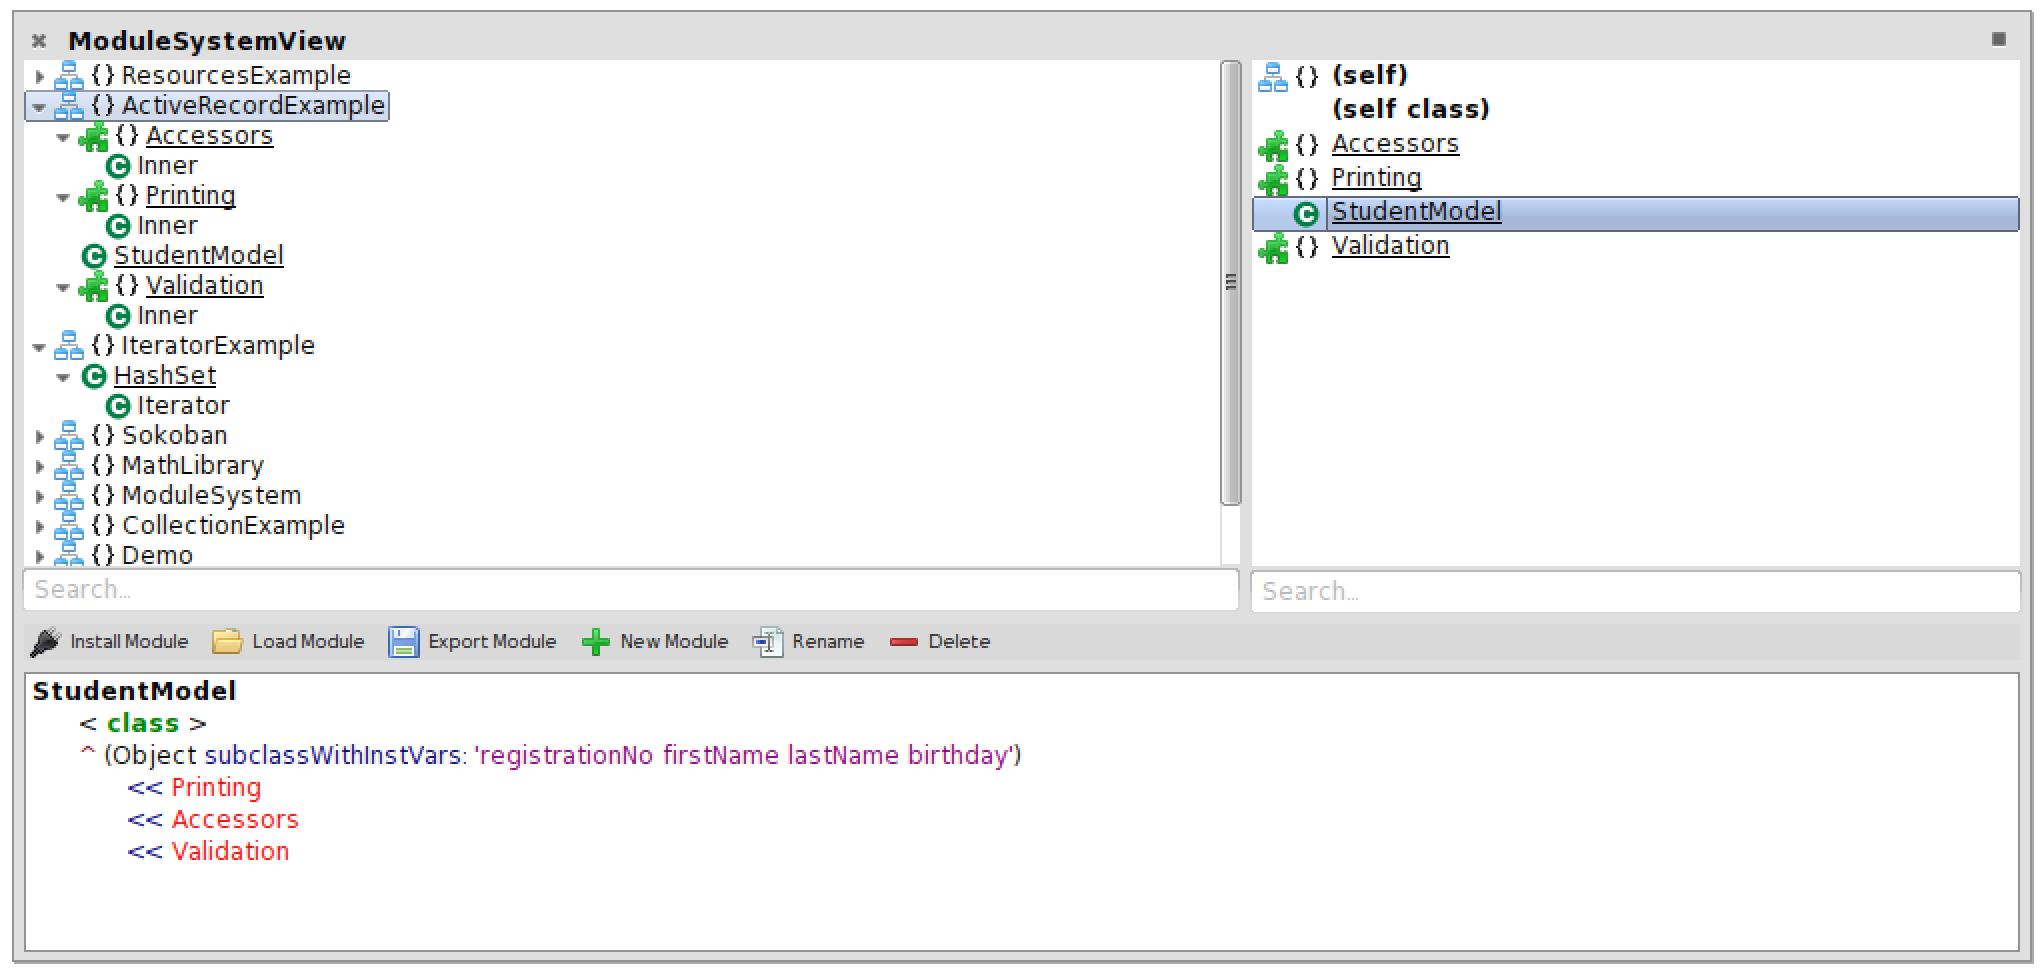
\includegraphics[width=\textwidth]{screenshot_classbrowser.png}
	\caption{Class Browser for Nested Classes}
	\label{fig:impl_class_browser}
\end{figure}

\msname is also integrated with the Squeak workspace and the test runner (Figure~\ref{fig:impl_integration}). Unit tests can be written and will show up in the test runner, as long as test classes are defined in a nested class called \texttt{Tests} within a top-level class. Later versions might traverse the entire nested classes graph to look for subclasses of \texttt{TestCase}, but this basic functionality allows us already to test parts of our system with code written in the system itself.

\begin{figure}[!htp]
	\centering
	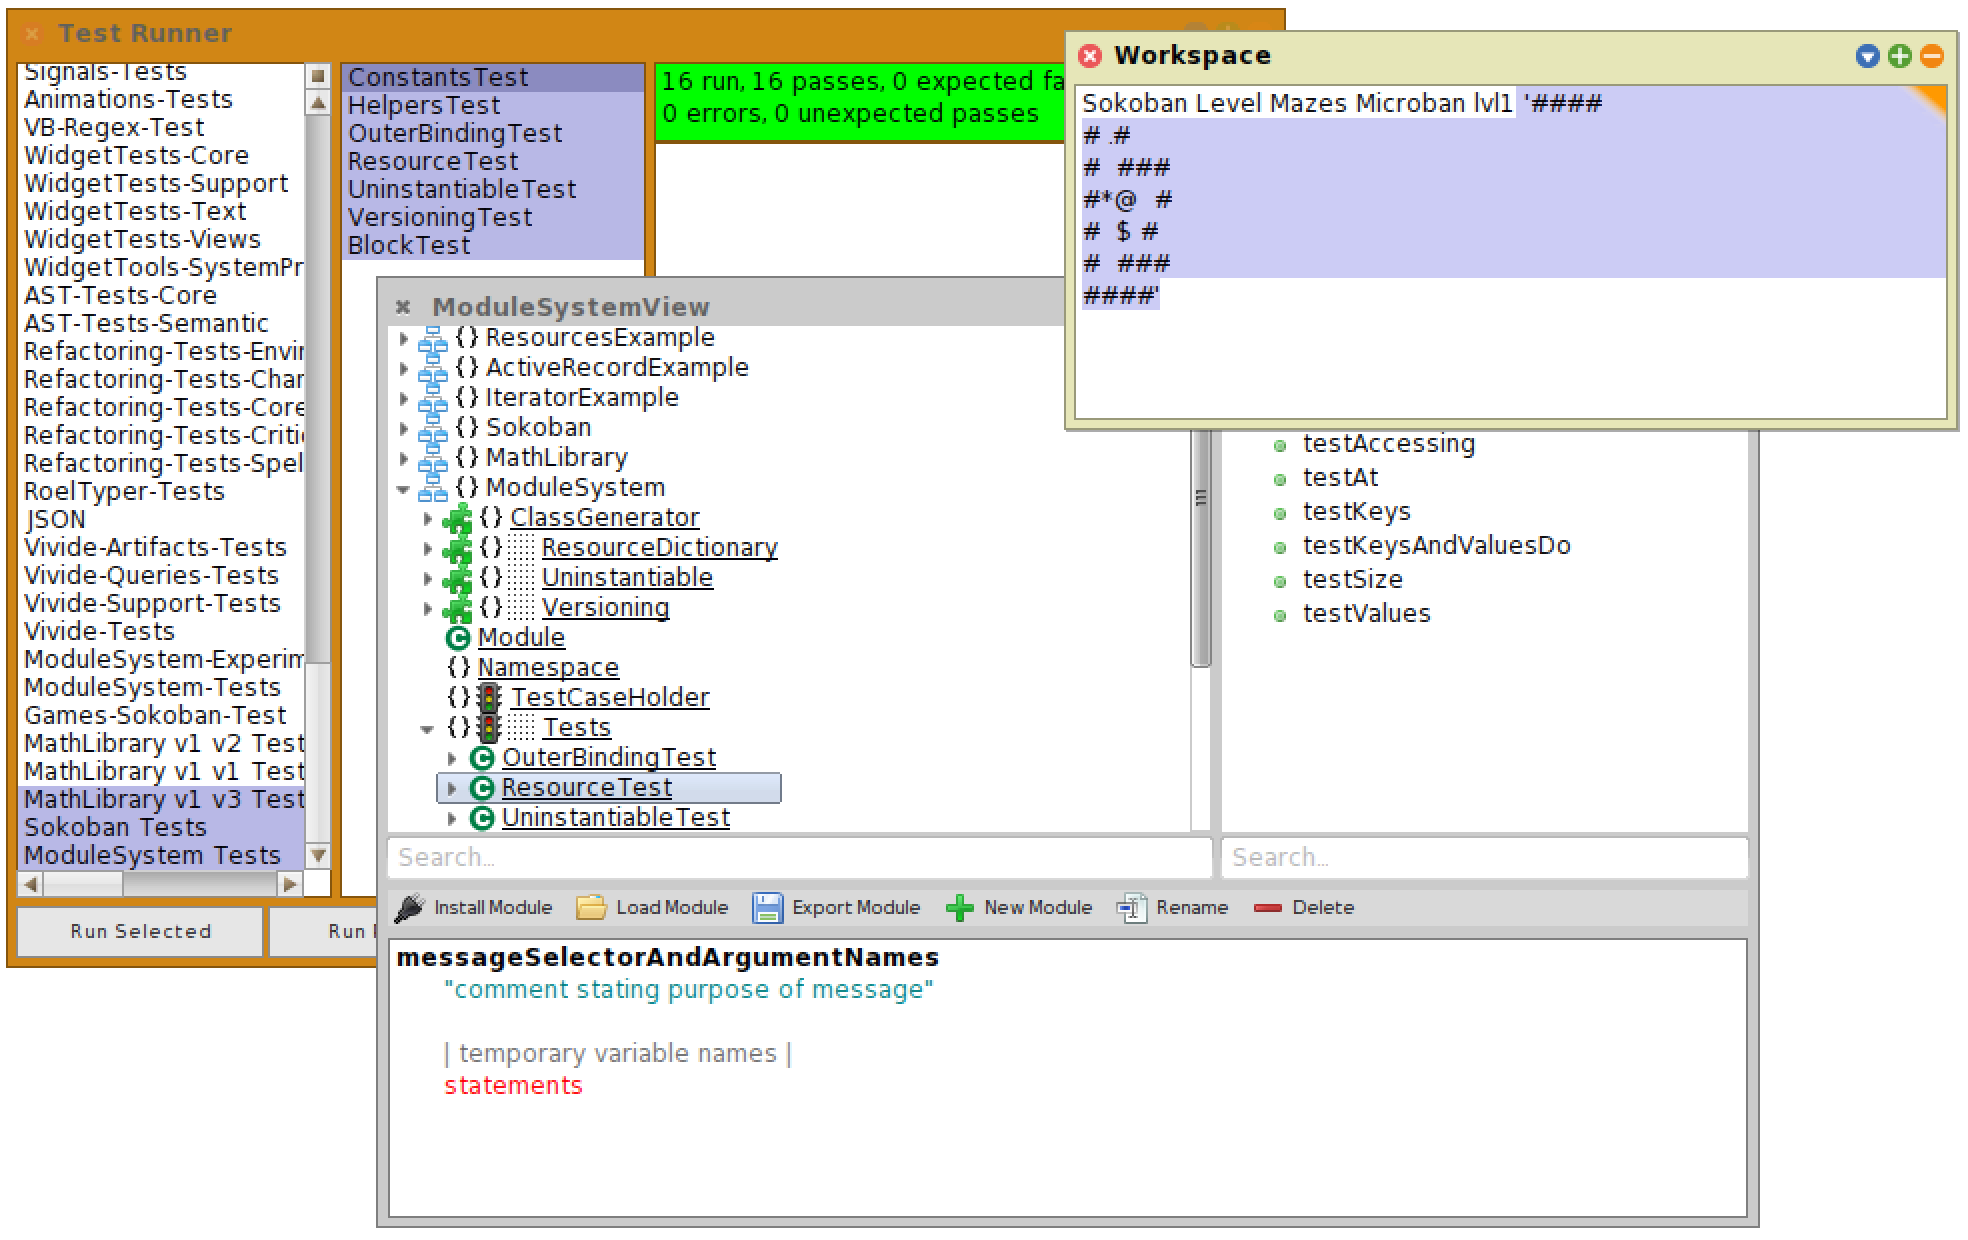
\includegraphics[width=\textwidth]{screenshot_integration.png}
	\caption{Integration in Squeak}
	\label{fig:impl_integration}
\end{figure}

\subsection{Debugger}
The Squeak debugger can be used to step through the source code. Parts of the source code can be selected and being evaluated. This also works with keywords that were introduced with \msname, such as \texttt{outer} and \texttt{enclosing}, because they are bound in the Squeak environment of the class.

What is still an issue is that the debugger shows slightly different source code from what the programmer wrote. For example, class references are prepended with the \texttt{scope} keyword. In addition, whenever the scope keyword is used, code must be inserted that generates a new instance of \texttt{LexicalScope}, because \texttt{scope} cannot be bound at compile time (see Section~\ref{sec:impl_keywords}). When stepping through the source code, the programmer will see additional stack frames for the class generator method and the class accessor method. The class accessor method is merely generated code, which is why it might be hidden in future versions of \msname.

Whenever the source code is changed in the debugger, the corresponding method specification is changed, causing all instantiations to be updated.

\section{Source Code Management}
Squeak uses Monticello as a source code packaging tool. Monticello can import and export code on a per-package basis. It can supports file system directories, HTTP URLs, and FTP URLs as repositories (i.e., the place where the code is loaded from and stored at). Whenever the programmer wants to get a new version of the source code, two options are available: packages can be loaded which will overwrite all local changes, and packages can be merged which will preserve local changes and only update new methods and classes. In case of merge conflicts, the programmer has to decide which version to load (old method or new method).

SqueakSource\footnote{http://www.squeaksource.com/} used to be a remote repository for Monticello projects (groups of packages). It is now deprecated and SmalltalkHub\footnote{http://www.smalltalkhub.com/} is one possible replacement.

\msname is not integrated with Monticello, because Monticello does currently not support class nesting. Many changes would be necessary in the import/export code, the user interface (e.g., merge window), and the backend repository; for example, SqueakSource allows browsing the code on its website, which does no longer work with class nesting.

\paragraph{Source Code Format}
\msname comes with its own import/export functionality and supports as only repository the file system as of now. The exported format is similar to the FileTree\footnote{https://github.com/dalehenrich/filetree} format. There is a directory for every class. Inside that directory, there are \texttt{instance} and \texttt{class} directories storing instance methods and class methods, respectively. For every nested class, the corresponding \texttt{class} directory contains a source code file for the class generator method and a directory for the nested class. For every method, there is a file containing its source code with the selector of the method as file name (colons are replaced with dots).

\begin{figure}[!htp]
\dirtree{%
.1 SpaceCleanup.st.
.1 \textbf{SpaceCleanup}.
.2 \textbf{instance}.
.2 \textbf{class}.
.3 Game.st.
.3 \textbf{Game}.
.4 \textbf{instance}.
.5 initialize.st.
.5 startGameWithPlayers..st.
.4 \textbf{class}.
.4 open.st.
}
\caption{Example: Source code export}
\label{fig:impl_source_export}
\end{figure}

Figure~\ref{fig:impl_source_export} illustrates what the exported format looks like. The top-level module is \texttt{SpaceCleanup}. It does not have any methods on the instance side, but a regular method \texttt{open} on class side, as well as a nested class \texttt{Game}. That nested class has instance methods \texttt{initialize} and \texttt{startGameWithPlayers:}.

\paragraph{Source Code Repository}
At the moment, we use git and GitHub to store modules written in our system, but any other external source code management system, such as Subversion or Mercurial, can be used. \msname does only support loading and saving, but not merging. It does also not store metadata associated with methods or classes, e.g., the author of a method or when it was changed. Instead, we rely on the underlying source code management system.

The following list gives an overview of how to load new changes into the system.
\begin{enumerate}
	\item Export local changes (if any).
	\item Get the latest source code from the remote repository (e.g., \texttt{git pull}).
	\item Resolve merge conflicts on the file system, if any.
	\item Import the entire module\footnote{This step only recompiles changed methods.}.
\end{enumerate}

The following list gives an overview of how local changes can be stored in a repository.
\begin{enumerate}
	\item Export the entire module.
	\item Get the latest source code from the remote repository (e.g., \texttt{git pull}).
	\item Resolve merge conflicts on the file system, if any.
	\item Send local working copy to the remote repository (e.g., \texttt{git commit} and \texttt{git push}).
\end{enumerate}
